\chapter{Introduction}

%Provide a context or background for the study (that is, the nature of the problem and its significance). State the specific purpose or research objective of, or hypothesis tested by, the study or observation. Cite only directly pertinent references, and do not include data or conclusions from the work being reported.

Deep Brain Stimulation (DBS) is a common treatment for advanced Parkinson's Disease (PD). In this therapeutic technique for PD, a small pair of electrodes is implanted surgically in a target area, subthalamic nucleus (STN) or the pars interna of Globus Pallidus (Gpi), to reverse motor symptoms through its stimulation. 

As the optimal positioning of the electrodes in the target area is of major importance for the best surgical results, clinicians decide the final electrodes position based on different approaches. Target coordinates are defined prior to surgery based on both patient's pre-operative magnetic resonance (MRI) and computed tomography (CT) imaging. During surgery, intra-operative microelectrode recordings (MER) along the trajectory to the target are visually inspected, and borders of STN and the area of interest are refined. Afterwards, final lead position is reviewed through therapeutic and side effects assessment by intra-operative stimulation. 

Specifically in DBS targetting STN, it is known that a proper placement of the final electrode and stimulation within the sensorimotor portion of STN is related with the best clinical results. However, it remains impossible to clearly identify this region on 1.5 Tesla MRI images and the features that can distinguish this region on MER remain to be clarified. 

Therefore, our aim in this study is to contribute for the development of clinical-decision support tools for target identification in STN-DBS, through computational analysis using intraoperative MER. 
%Objectives are deeply explained in section~\ref{sec:objectives}, but theoretical background regarding Parkinson's Disease and STN-DBS is presented in the following section in order to provide better understanding of the problem and purpose. %followed by our objectives, work-flow and related work. 

%\textit{Is it better to present objectives here or as a separate chapter?}

%However, this process can be time-consuming making the development of clinical-decision support tools a major need in this field.  

\section{Theoretical background}

In this section, theoretical information regarding Parkinson's Disease and Deep Brain Stimulation targetting STN (STN-DBS) is presented in order to provide better understanding of the problem and purpose of our study.

\subsection{Parkinson's Disease}
Parkinson's Disease is the second most common neurological disease worldwide. It is a neurodegenerative, chronic and progressive disease and its annual incidence is thought to be 15 per 100,000 according to \citeA{Tysnes2017}. Its prevalence increases with age, 1 \% of population over 60 years old suffers PD, and genetic factors are thought to be involved in 5–10\% of the cases

"It is generally considered that known genetic causes may be relevant in more than 5\% of the total PD population and that monogenetic causes are rare, but some propose that monogenetic causes may be involved in as many as 5–10\% of the PD population (Lill 2016)", Tysnes2017

. Altough its cause is unknow in most cases, several environmental factors are related with increased risk of PD. Previous studies also present higher incidence rate of PD in men than women \cite{Tysnes2017, Wooten2004}. \\

\textbf{Symptomatology}

Parkinson's Disease symptoms are both motor and non-motor related and can be categorized into 5 groups according to \citeA{Maiti2017}: early symptoms, primary and secondary both motor and non-motor related. 
Early symptoms are progressive and slight, which may lead in difficulties for PD diagnosis, such as posture difficulty, mild tremors, soft speech or lose track of thoughs or words among others.  Tremors, muscle stiffness (rigidity), slowness of movement (bradykinesia), absence of  movement (akinesia) and decreased bodily movement (hypokinesia) are some of the primary motor characteristics in PD. In contrast, secondary motor symptoms are such as sexual dysfunction, dystonia or difficulty in swallowing and chewing. Regarding primary non-motor symptoms, depression, dementia, cognitive dysfunction and/or sleep disorders occur frequently. Secondary non-motor symptoms are related with gesture and emotional variations, sweating, urinary problems or hypotension. 
\\
 
%parkisonism é um conjunto de alteraciones, que não só são causadas por o PD, tamen por enfermidades vasculares ou heredo-degenerativos entre outros.
%acinésia (bradicinésia): dificultade em iniciar o movemento e diminucion progressiva da velocidade, rigidez, tremor de repouso, aalteraçoes posturais e de marcha
%sintomas nao motores:
%hiposmia, disautonomia, alteraçoes do sono, deterioraça cognitiva, depresao, apatia ansiedade, fatiga e dor e alteraçoes psicoticas (que tenden a surgir ao fimde alguns anos após o surgimento dos sintomas motores

\textbf{Mechanism underlying PS symptoms}

Basal ganglia refers to a group of  interconnected subcortical structures, which play an important role mainly in motor control but also non-motor related roles such as executive functions, behaviour or emotions. Subthalamic nucleus, substantia nigra pars compacta (SNc), globus pallidus (GPi and GPe; internal and external respectively), and dorsal striatum (with both caudate nucleus and putamen) are the main nuclei in the basal ganglia \cite{Fahn2011} .%citeLanciego2012_functionalNeuroanatomyBasalGanglia
In order to control execution of movements, motor information is modulated by the combination of an excitatory or direct pathway, and an inhibitory or indirect pathway through basal ganglia structures and cortex, as a closed circuit illustrated in figure~\ref{fig:basalGanglia}.

\begin{figure}[!htb]
     \centering    
         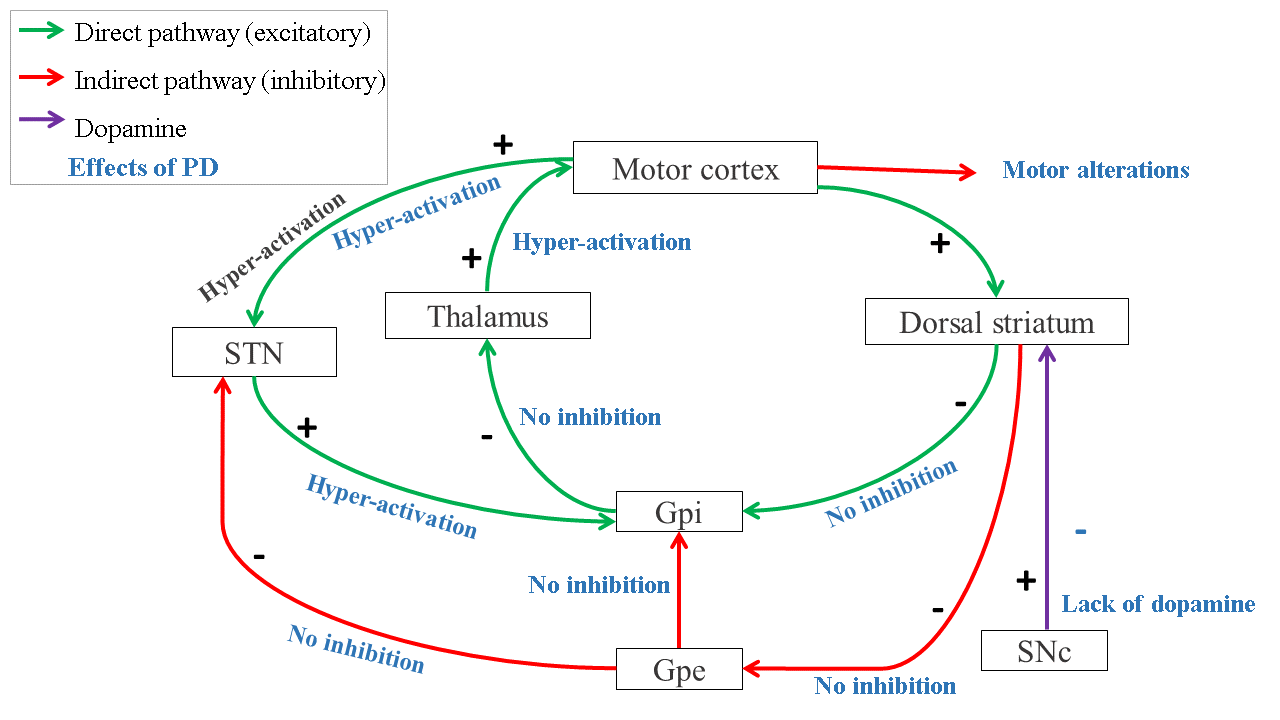
\includegraphics[width=0.9\textwidth]{basalGangliacircuit.png} 
       \caption{Neural network between main basal ganglia structures with connecting pathways inhibitory, in red, and excitatory in green. Alterations on pathways in PD patients are indicated in blue.}
     \label{fig:basalGanglia}
\end{figure} 

Parkinson's Disease is characterized by progressive degeneration of neurons in substantia nigra pars compacta (SNc), decreasing the secretion of dopamine (DA), an essential brain monoamine which regulates the excitability of striatal neurons. 
Effects of loss of DA lead to alterations in neuronal activity resulting in difficulties for movement control and are present both in indirect and direct pathways, as indicated in blue in  figure \ref{fig:basalGanglia}. Consequently GPi is inhibited and increases inhibition signals in the thalamus, finally hyper-activating the motor cortex and consequently inhibiting the control of voluntary movements \cite{Maiti2017}.% that hyper-ac which and results in inhibition of voluntary movement control, in motor cortex.  
\\

\textbf{Treatments for Parkinson's Disease}

Different therapies are currently available for the treatment of motor symptoms in PD. At the present, both medication and surgery are the most frequently used therapies to treat PD symptoms ((or decrease progression)), but new promising treatments are emerging and  being studied such as stem cell transplantation or gene therapy \cite{Maiti2017}.

During early stages of PD treatment, medication typically is the best option to control motor symptoms. Most common used drug is Levodopa (L-dopa) which is a dopaminergic drug that decreases the SNc degeneration by improving its dopamine levels. Nevertheless, since increment of dopamine occurs in other brain regions beyond the basal ganglia, it may generate adverse effects, specially in long-term treatments, such as motor fluctuations or dyskinesias. Also other types of drugs are used in PD treatment to treat motor (dopaminergic and non-dopaminergic drugs) and non-motor symptons.

For patients with motor symptoms refractory to the best medical therapy different therapeutical approaches are tried: usually deep brain stimulation or lesion surgery. 
 Lesion surgeries for PD are known as pallidotomy and thalamotomy referring to the respective surgically destroyed part, globus pallidus and thalamus. Motor symptoms decrease with these procedures since inhibitory neural activity of these estructures was increased. Nevertheless, since lesion surgery is irreversible and lesions in adjacent areas may occur, electrical neuro stimulation surgery (Deep Brain Stimulation) is a good alternative and currently most commonly used for PD.
 
%Motor fluctuations, change between states of regarding the control of motor symptoms. "off-time", "on-time"

\subsection{Deep Brain Stimulation}

Deep Brain Stimulation (DBS) is a surgical treatment for refractory movement disorders, such as PD, dystonia or tremors. A target area of the brain is stimulated through surgically-implanted electrodes to reverse motor symptoms by inducing neuronal activity alterations.

\begin{figure}[!htb]
     \centering    
         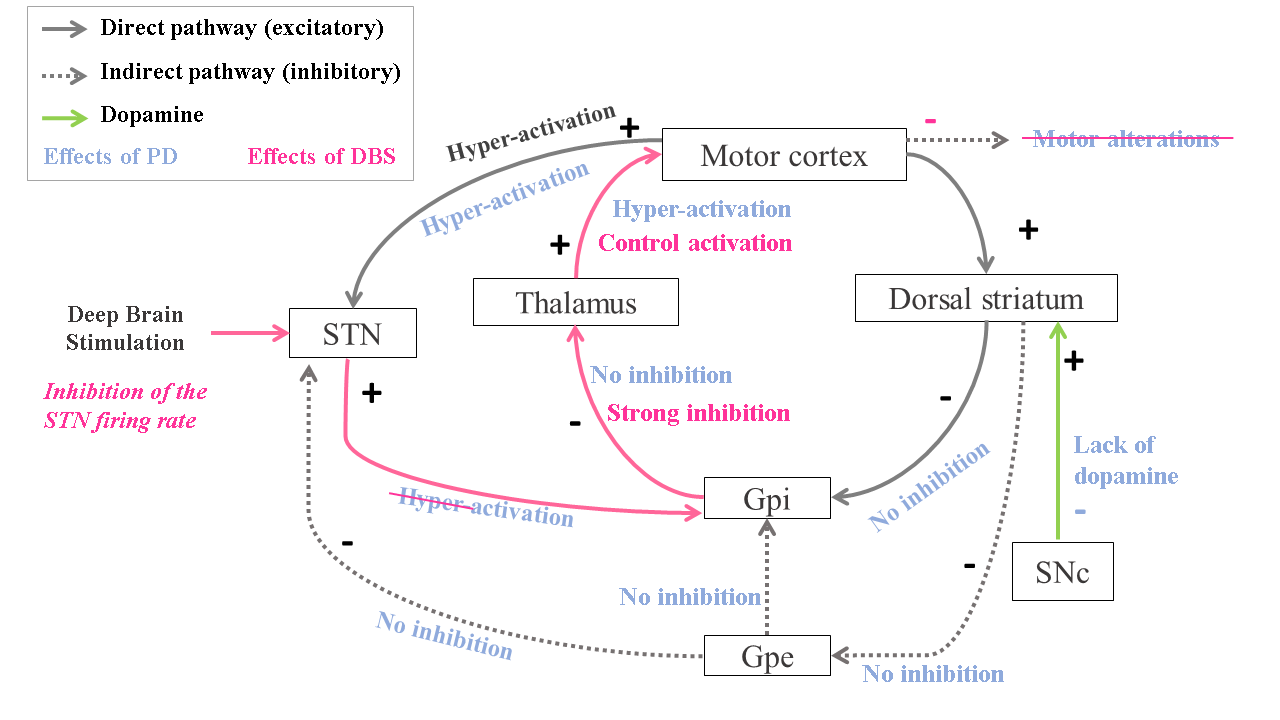
\includegraphics[width=0.9\textwidth]{basalGangliacircuitDBS.png} 

       \caption{Basal ganglia circuitry with alterations induced by STN-DBS in both indirect and direct pathways. Alterations to both inhibitory and excitatory pathways in PD patients are indicated in blue.}
     \label{fig:basalGangliaDBS}
\end{figure}

Our study is focused on STN-DBS and therefore our stimulation target is STN, typically used for PD treatment along with GPi. Up to 20\% of PD patients are considered suitable candidates for Deep Brain Stimulation (DBS),\textit{ since DEVELOP ABOUT CANDIDATE CONDITIONS FOR DBS?.} \cite{WagleShukla2014}.
% paf 45 vaz 

%\cite{Hamani2017} \cite{Tysnes2017}
%Condiciones para ser candidato para PD: pagina 45 vaz

Mechanism underlying STN-DBS can be explained following with the basal ganglia circuitry, figure~\ref{fig:basalGanglia}, altough it is still fully unclear how mechanism underlying STN-DBS exactly work within the brain. As illustrated in the basal ganglia neural network in figure~\ref{fig:basalGangliaDBS}, artificial stimulation in the hyper-activated STN provokes an inhibition of its firing rate that activates the GPi, consequently inhibiting the thalamus and improving movement control from motor cortex \cite{Maiti2017, Gradinaru2009, Negida2018}.

Subthalamic Nucleus is divided into three functional regions: sensorimotor, limbic and associative, which are located in dorsolateral, anteroventral and medial territories respectively, and it is part of a bigger functional structure called the basal Ganglia as mentioned before. Previous studies suggest that precise positioning of the electrode and stimulation within the sensorimotor part of the STN is of mayor importance for optimal results and to avoid side effects \cite{Castrioto2014, Wodarg2012, Johnsen2010}. However, identification of sensorimotor STN region based on 1.5 Tesla MRI images is impossible and still unclear based on MER characteristics.

\textit{Outcomes?}

\subsubsection{DBS procedure}
Previously to surgery and stereotactic frame implantation, pre-operative magnetic resonance imaging (MRI) is acquired in order to subsequently plan the lead trajectory based on the patient's anatomy. After installation of stereotactic frame, pre-implantation contrast-enhanced computed tomography (CT) is performed on patient, which displays a reference scale through its ferromagnetic materials.

Estimation of STN target coordinates is based on both CT and MRI pre-operative images co-registered and its fiducial points, AC (anterior commisure) and PC (posterior commisure).  For both hemispheres (one at a time), different trajectories and strategies are discussed and visualized to achieve the best trajectory based on merged images in both three views (sagital, coronal, axial) and also as \textit{probe view}, which facilitates avoiding problematic trajectories. Best electrode's trajectory avoids white matter, critical cerebral tissue, veins or other conflict points.

Once target coordinates are selected, surgery is performed one hemisphere at a time. Stereotactic frame is configured according to the target coordinates and after burr hole trepanations, electrodes are connected and implanted into the brain according to the fixed coordinates in the frame. In our study using Medtronic 3389 electrodes, only central, lateral and anterior leads were implanted but up to 7 leads in each electrode are available to use.

Registration of micro electrode recordings (MER) is next performed in order to identificate STN and therefore the best position based on acquired signals from different depths. MER start when electrodes are positioned one centimeter above the planned target, and recordings are acquired at different depths to target simultaneously for all the channels, located with a parallel trajectory to the center lead. \textit{(Through Medtronic console )}
According to the acquired signal and based on visual inspection and experience of the neurologist, region of brain in which the electrode is located for each depth is identified in a table. After registration of all depths, kind of a reconstruction of the shape of the target is estimated based on MER annotations and possible definitive target coordinates are determined.
 
Intraoperative stimulation is then executed in order to refine the final localization of lead based on therapeutic and side effects assessment. Different estimated points of interest are stimulated through inserted macro-electrodes with gradual variations of both intensities and frequency. Once stimulation effects, such as eye or muscle contractions, are assessed and the best position is determined, definitive electrode is implanted.
 
Second part of surgery includes the implementation of the neurostimulatter with the battery in the patient and its connection to the electrodes as illustrated in figure 1.1 \cite{Medtronic2007}. Batteries may need to be replaced in 3 to 5 years depending on the patient and stimulation parameters. 

\begin{figure}[!htb]
     \centering    
         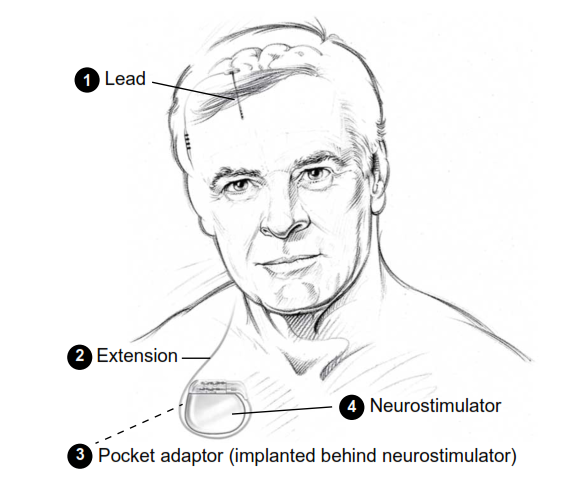
\includegraphics[width=0.6\textwidth]{medtronicDBScomp.png} 

       \caption{Medtronic DBS System Components. \small{From Medtronic.}}
     \label{fig:medtronicDBS}
\end{figure}

\textit{Develop about DBS programming??}

\subsection{Electrophisiology or action potentials}
\label{sec:electroph}
Explaining STN localisation and typical waveforms through different parts of the brain?
Also differences between patients and characteristics in PD (STN) or is it better in the discussion?

\subsection{Classification}

\section{Objectives}
\label{sec:objectives}
Development of clinical-support tools for identification of the target area in DBS is important for this field. As mentioned before, positioning of final electrodes in the precise location is related with the best therapeutic results and its definition depends on the neurologists expertise among other factors, so it is a time-consuming and subjective process. In this study we aim to contribute to the development of computational tools that can assist clinical decision in target identification in STN-DBS. Therefore, we split our objectives into four main tasks:

\begin{enumerate}
\item Development of an unbiased unsupervised tool for signal processing, analysis and feature extraction to distinguish STN from non-STN intraoperative MER, but easily adaptable for other types of signals and regions.

\item Development of an automatic approach for spike sorting and signal analysis of human brain MER to study physiological properties of neurons. We aim to construct this tool generalizable to other brain regions and unsupervised through the adjustment of existing algorithms to our approach.

\item Identification of features that distinguish sensorimotor subdivision of STN vs. limbic and associative using extracted features from both previously constructed tools.

\item Development of a hybrid unsupervised/supervised machine learning classification approach that uses extracted MER features for high-accuracy identification of STN. This approach can be optimized using individual patient lead trajectory localization reconstruction based on imagiology, fused with an STN functional subdivision atlas.
\end{enumerate}

\section{Contributions}